% Options for packages loaded elsewhere
\PassOptionsToPackage{unicode}{hyperref}
\PassOptionsToPackage{hyphens}{url}
\PassOptionsToPackage{dvipsnames,svgnames,x11names}{xcolor}
%
\documentclass[
  a4paper,
]{article}

\usepackage{amsmath,amssymb}
\usepackage{lmodern}
\usepackage{iftex}
\ifPDFTeX
  \usepackage[T1]{fontenc}
  \usepackage[utf8]{inputenc}
  \usepackage{textcomp} % provide euro and other symbols
\else % if luatex or xetex
  \usepackage{unicode-math}
  \defaultfontfeatures{Scale=MatchLowercase}
  \defaultfontfeatures[\rmfamily]{Ligatures=TeX,Scale=1}
\fi
% Use upquote if available, for straight quotes in verbatim environments
\IfFileExists{upquote.sty}{\usepackage{upquote}}{}
\IfFileExists{microtype.sty}{% use microtype if available
  \usepackage[]{microtype}
  \UseMicrotypeSet[protrusion]{basicmath} % disable protrusion for tt fonts
}{}
\makeatletter
\@ifundefined{KOMAClassName}{% if non-KOMA class
  \IfFileExists{parskip.sty}{%
    \usepackage{parskip}
  }{% else
    \setlength{\parindent}{0pt}
    \setlength{\parskip}{6pt plus 2pt minus 1pt}}
}{% if KOMA class
  \KOMAoptions{parskip=half}}
\makeatother
\usepackage{xcolor}
\usepackage[top=30mm,left=20mm,heightrounded]{geometry}
\setlength{\emergencystretch}{3em} % prevent overfull lines
\setcounter{secnumdepth}{5}
% Make \paragraph and \subparagraph free-standing
\ifx\paragraph\undefined\else
  \let\oldparagraph\paragraph
  \renewcommand{\paragraph}[1]{\oldparagraph{#1}\mbox{}}
\fi
\ifx\subparagraph\undefined\else
  \let\oldsubparagraph\subparagraph
  \renewcommand{\subparagraph}[1]{\oldsubparagraph{#1}\mbox{}}
\fi

\usepackage{color}
\usepackage{fancyvrb}
\newcommand{\VerbBar}{|}
\newcommand{\VERB}{\Verb[commandchars=\\\{\}]}
\DefineVerbatimEnvironment{Highlighting}{Verbatim}{commandchars=\\\{\}}
% Add ',fontsize=\small' for more characters per line
\usepackage{framed}
\definecolor{shadecolor}{RGB}{241,243,245}
\newenvironment{Shaded}{\begin{snugshade}}{\end{snugshade}}
\newcommand{\AlertTok}[1]{\textcolor[rgb]{0.68,0.00,0.00}{#1}}
\newcommand{\AnnotationTok}[1]{\textcolor[rgb]{0.37,0.37,0.37}{#1}}
\newcommand{\AttributeTok}[1]{\textcolor[rgb]{0.40,0.45,0.13}{#1}}
\newcommand{\BaseNTok}[1]{\textcolor[rgb]{0.68,0.00,0.00}{#1}}
\newcommand{\BuiltInTok}[1]{\textcolor[rgb]{0.00,0.23,0.31}{#1}}
\newcommand{\CharTok}[1]{\textcolor[rgb]{0.13,0.47,0.30}{#1}}
\newcommand{\CommentTok}[1]{\textcolor[rgb]{0.37,0.37,0.37}{#1}}
\newcommand{\CommentVarTok}[1]{\textcolor[rgb]{0.37,0.37,0.37}{\textit{#1}}}
\newcommand{\ConstantTok}[1]{\textcolor[rgb]{0.56,0.35,0.01}{#1}}
\newcommand{\ControlFlowTok}[1]{\textcolor[rgb]{0.00,0.23,0.31}{#1}}
\newcommand{\DataTypeTok}[1]{\textcolor[rgb]{0.68,0.00,0.00}{#1}}
\newcommand{\DecValTok}[1]{\textcolor[rgb]{0.68,0.00,0.00}{#1}}
\newcommand{\DocumentationTok}[1]{\textcolor[rgb]{0.37,0.37,0.37}{\textit{#1}}}
\newcommand{\ErrorTok}[1]{\textcolor[rgb]{0.68,0.00,0.00}{#1}}
\newcommand{\ExtensionTok}[1]{\textcolor[rgb]{0.00,0.23,0.31}{#1}}
\newcommand{\FloatTok}[1]{\textcolor[rgb]{0.68,0.00,0.00}{#1}}
\newcommand{\FunctionTok}[1]{\textcolor[rgb]{0.28,0.35,0.67}{#1}}
\newcommand{\ImportTok}[1]{\textcolor[rgb]{0.00,0.46,0.62}{#1}}
\newcommand{\InformationTok}[1]{\textcolor[rgb]{0.37,0.37,0.37}{#1}}
\newcommand{\KeywordTok}[1]{\textcolor[rgb]{0.00,0.23,0.31}{#1}}
\newcommand{\NormalTok}[1]{\textcolor[rgb]{0.00,0.23,0.31}{#1}}
\newcommand{\OperatorTok}[1]{\textcolor[rgb]{0.37,0.37,0.37}{#1}}
\newcommand{\OtherTok}[1]{\textcolor[rgb]{0.00,0.23,0.31}{#1}}
\newcommand{\PreprocessorTok}[1]{\textcolor[rgb]{0.68,0.00,0.00}{#1}}
\newcommand{\RegionMarkerTok}[1]{\textcolor[rgb]{0.00,0.23,0.31}{#1}}
\newcommand{\SpecialCharTok}[1]{\textcolor[rgb]{0.37,0.37,0.37}{#1}}
\newcommand{\SpecialStringTok}[1]{\textcolor[rgb]{0.13,0.47,0.30}{#1}}
\newcommand{\StringTok}[1]{\textcolor[rgb]{0.13,0.47,0.30}{#1}}
\newcommand{\VariableTok}[1]{\textcolor[rgb]{0.07,0.07,0.07}{#1}}
\newcommand{\VerbatimStringTok}[1]{\textcolor[rgb]{0.13,0.47,0.30}{#1}}
\newcommand{\WarningTok}[1]{\textcolor[rgb]{0.37,0.37,0.37}{\textit{#1}}}

\providecommand{\tightlist}{%
  \setlength{\itemsep}{0pt}\setlength{\parskip}{0pt}}\usepackage{longtable,booktabs,array}
\usepackage{calc} % for calculating minipage widths
% Correct order of tables after \paragraph or \subparagraph
\usepackage{etoolbox}
\makeatletter
\patchcmd\longtable{\par}{\if@noskipsec\mbox{}\fi\par}{}{}
\makeatother
% Allow footnotes in longtable head/foot
\IfFileExists{footnotehyper.sty}{\usepackage{footnotehyper}}{\usepackage{footnote}}
\makesavenoteenv{longtable}
\usepackage{graphicx}
\makeatletter
\def\maxwidth{\ifdim\Gin@nat@width>\linewidth\linewidth\else\Gin@nat@width\fi}
\def\maxheight{\ifdim\Gin@nat@height>\textheight\textheight\else\Gin@nat@height\fi}
\makeatother
% Scale images if necessary, so that they will not overflow the page
% margins by default, and it is still possible to overwrite the defaults
% using explicit options in \includegraphics[width, height, ...]{}
\setkeys{Gin}{width=\maxwidth,height=\maxheight,keepaspectratio}
% Set default figure placement to htbp
\makeatletter
\def\fps@figure{htbp}
\makeatother
\newlength{\cslhangindent}
\setlength{\cslhangindent}{1.5em}
\newlength{\csllabelwidth}
\setlength{\csllabelwidth}{3em}
\newlength{\cslentryspacingunit} % times entry-spacing
\setlength{\cslentryspacingunit}{\parskip}
\newenvironment{CSLReferences}[2] % #1 hanging-ident, #2 entry spacing
 {% don't indent paragraphs
  \setlength{\parindent}{0pt}
  % turn on hanging indent if param 1 is 1
  \ifodd #1
  \let\oldpar\par
  \def\par{\hangindent=\cslhangindent\oldpar}
  \fi
  % set entry spacing
  \setlength{\parskip}{#2\cslentryspacingunit}
 }%
 {}
\usepackage{calc}
\newcommand{\CSLBlock}[1]{#1\hfill\break}
\newcommand{\CSLLeftMargin}[1]{\parbox[t]{\csllabelwidth}{#1}}
\newcommand{\CSLRightInline}[1]{\parbox[t]{\linewidth - \csllabelwidth}{#1}\break}
\newcommand{\CSLIndent}[1]{\hspace{\cslhangindent}#1}

\usepackage[noblocks]{authblk}
\renewcommand*{\Authsep}{, }
\renewcommand*{\Authand}{, }
\renewcommand*{\Authands}{, }
\renewcommand\Affilfont{\small}
\makeatletter
\makeatother
\makeatletter
\makeatother
\makeatletter
\@ifpackageloaded{caption}{}{\usepackage{caption}}
\AtBeginDocument{%
\ifdefined\contentsname
  \renewcommand*\contentsname{Table of contents}
\else
  \newcommand\contentsname{Table of contents}
\fi
\ifdefined\listfigurename
  \renewcommand*\listfigurename{List of Figures}
\else
  \newcommand\listfigurename{List of Figures}
\fi
\ifdefined\listtablename
  \renewcommand*\listtablename{List of Tables}
\else
  \newcommand\listtablename{List of Tables}
\fi
\ifdefined\figurename
  \renewcommand*\figurename{Figure}
\else
  \newcommand\figurename{Figure}
\fi
\ifdefined\tablename
  \renewcommand*\tablename{Table}
\else
  \newcommand\tablename{Table}
\fi
}
\@ifpackageloaded{float}{}{\usepackage{float}}
\floatstyle{ruled}
\@ifundefined{c@chapter}{\newfloat{codelisting}{h}{lop}}{\newfloat{codelisting}{h}{lop}[chapter]}
\floatname{codelisting}{Listing}
\newcommand*\listoflistings{\listof{codelisting}{List of Listings}}
\makeatother
\makeatletter
\@ifpackageloaded{caption}{}{\usepackage{caption}}
\@ifpackageloaded{subcaption}{}{\usepackage{subcaption}}
\makeatother
\makeatletter
\@ifpackageloaded{tcolorbox}{}{\usepackage[many]{tcolorbox}}
\makeatother
\makeatletter
\@ifundefined{shadecolor}{\definecolor{shadecolor}{rgb}{.97, .97, .97}}
\makeatother
\makeatletter
\makeatother
\ifLuaTeX
  \usepackage{selnolig}  % disable illegal ligatures
\fi
\IfFileExists{bookmark.sty}{\usepackage{bookmark}}{\usepackage{hyperref}}
\IfFileExists{xurl.sty}{\usepackage{xurl}}{} % add URL line breaks if available
\urlstyle{same} % disable monospaced font for URLs
\hypersetup{
  pdftitle={INLABru : Convenient digital soil mapping model fitting using INLA-SPDE},
  pdfauthor={Nicolas Saby; Thomas Opitz},
  colorlinks=true,
  linkcolor={blue},
  filecolor={Maroon},
  citecolor={Blue},
  urlcolor={Blue},
  pdfcreator={LaTeX via pandoc}}

\title{INLABru : Convenient digital soil mapping model fitting using
INLA-SPDE}
\author{Nicolas Saby \and Thomas Opitz}
\date{4/24/23}

\begin{document}
\maketitle
\ifdefined\Shaded\renewenvironment{Shaded}{\begin{tcolorbox}[breakable, frame hidden, interior hidden, borderline west={3pt}{0pt}{shadecolor}, sharp corners, enhanced, boxrule=0pt]}{\end{tcolorbox}}\fi

\renewcommand*\contentsname{Table of contents}
{
\hypersetup{linkcolor=}
\setcounter{tocdepth}{3}
\tableofcontents
}
\hypertarget{introduction}{%
\section{Introduction}\label{introduction}}

Pedometricians are nowadays big fans of machine learning (ML) approaches
with on the top the widely used random forest algorithm, see for example
(L. Poggio et al. 2021). These algorithms are indeed particularly
adapted to the management of large data sets to map soil properties on
wide extent in a large range of situations. The techniques are based on
classification and regression, but they take no account of spatial
correlations (Heuvelink and Webster 2022). This trend also seems to be
accompanied by a lesser use of geostatistical techniques that maybe
require more computer resource and statistical skills. However, if
prediction is performed in several steps (\emph{eg} regression or any
other machine learning prediction in step 1, followed by spatial kriging
of the residuals in step 2), then an accurate assessment of the
prediction uncertainties is difficult since uncertainties from the first
step must be propagated through to the second step.

In this paper, we propose to solve these issues by using the fully
Bayesian estimation framework based on the integrated nested Laplace
approximation (INLA,(Rue, Martino, and Chopin 2009)), combined with the
so-called stochastic partial differential equation approach (SPDE,
Lindgren, Rue, and Lindström 2011) providing numerically convenient
representations of Gaussian processes over continuous space. The INLA
method is an alternative to traditional Markov chain Monte Carlo methods
for Bayesian estimation and provides off-the-shelf implementation of
fast and accurate deterministic approximations of posterior inferences
for a large class of models. INLA with SPDE is handle to handle very
large data sets.

INLA-SPDE was already introduced by (Laura Poggio et al. 2016) or (Huang
2017) in the pedometrics community. However, the use of this approach
was probably hindered by the complexity of the INLA R package. Recently,
the \texttt{INLABru} R package (Yuan et al. 2017) originally developed
for the point process models has integrates a range of functions to help
in implementing INLA-SPDE models in a convenient way. We propose here to
show you using a simple and classical regression kriging approach as an
example.

When the number of data is huge, it is important to mention that one can
improve the performance by using the PARDISO solver. Please, go to
https://www.pardiso-project.org/r-inla/\#license to apply for a license.
Also, use inla.pardiso() for instructions on how to enable the PARDISO
sparse library.

\hypertarget{set-up}{%
\section{Set up}\label{set-up}}

\hypertarget{load-packages}{%
\subsection{Load packages}\label{load-packages}}

We use here a set of R packages in the list below.

The latest version of R (eg \textgreater4.2) should be installed on your
computer for \texttt{INLABru}.

\begin{Shaded}
\begin{Highlighting}[]
\FunctionTok{library}\NormalTok{(INLA)}
\FunctionTok{library}\NormalTok{(inlabru)}
\FunctionTok{library}\NormalTok{(dplyr)}
\FunctionTok{library}\NormalTok{(tmap)}
\FunctionTok{library}\NormalTok{(gstat) }\CommentTok{\# for the meuse data}
\FunctionTok{library}\NormalTok{(tmap)}
\FunctionTok{library}\NormalTok{(ggplot2)}
\end{Highlighting}
\end{Shaded}

The \texttt{INLABru} method is a wrapper for \texttt{INLA::inla} and
provides multiple enhancements.

\hypertarget{point-data-and-rasters}{%
\subsection{Point data and rasters}\label{point-data-and-rasters}}

We use the open data \texttt{meuse} from the \texttt{gstat} package

\begin{Shaded}
\begin{Highlighting}[]
\FunctionTok{data}\NormalTok{(meuse)}
\FunctionTok{data}\NormalTok{(meuse.grid)}

\FunctionTok{str}\NormalTok{(meuse)}
\end{Highlighting}
\end{Shaded}

\begin{verbatim}
'data.frame':   155 obs. of  14 variables:
 $ x      : num  181072 181025 181165 181298 181307 ...
 $ y      : num  333611 333558 333537 333484 333330 ...
 $ cadmium: num  11.7 8.6 6.5 2.6 2.8 3 3.2 2.8 2.4 1.6 ...
 $ copper : num  85 81 68 81 48 61 31 29 37 24 ...
 $ lead   : num  299 277 199 116 117 137 132 150 133 80 ...
 $ zinc   : num  1022 1141 640 257 269 ...
 $ elev   : num  7.91 6.98 7.8 7.66 7.48 ...
 $ dist   : num  0.00136 0.01222 0.10303 0.19009 0.27709 ...
 $ om     : num  13.6 14 13 8 8.7 7.8 9.2 9.5 10.6 6.3 ...
 $ ffreq  : Factor w/ 3 levels "1","2","3": 1 1 1 1 1 1 1 1 1 1 ...
 $ soil   : Factor w/ 3 levels "1","2","3": 1 1 1 2 2 2 2 1 1 2 ...
 $ lime   : Factor w/ 2 levels "0","1": 2 2 2 1 1 1 1 1 1 1 ...
 $ landuse: Factor w/ 15 levels "Aa","Ab","Ag",..: 4 4 4 11 4 11 4 2 2 15 ...
 $ dist.m : num  50 30 150 270 380 470 240 120 240 420 ...
\end{verbatim}

\begin{Shaded}
\begin{Highlighting}[]
\FunctionTok{str}\NormalTok{(meuse.grid)}
\end{Highlighting}
\end{Shaded}

\begin{verbatim}
'data.frame':   3103 obs. of  7 variables:
 $ x     : num  181180 181140 181180 181220 181100 ...
 $ y     : num  333740 333700 333700 333700 333660 ...
 $ part.a: num  1 1 1 1 1 1 1 1 1 1 ...
 $ part.b: num  0 0 0 0 0 0 0 0 0 0 ...
 $ dist  : num  0 0 0.0122 0.0435 0 ...
 $ soil  : Factor w/ 3 levels "1","2","3": 1 1 1 1 1 1 1 1 1 1 ...
 $ ffreq : Factor w/ 3 levels "1","2","3": 1 1 1 1 1 1 1 1 1 1 ...
\end{verbatim}

The first action is to create \texttt{sp} objects:

\begin{itemize}
\item
  a \texttt{SpatialPointsDataFrame} corresponding to the regression
  matrix and,
\item
  the prediction grid
\end{itemize}

\begin{Shaded}
\begin{Highlighting}[]
\FunctionTok{coordinates}\NormalTok{(meuse) }\OtherTok{\textless{}{-}} \FunctionTok{c}\NormalTok{(}\StringTok{\textquotesingle{}x\textquotesingle{}}\NormalTok{,}\StringTok{\textquotesingle{}y\textquotesingle{}}\NormalTok{)}

\FunctionTok{coordinates}\NormalTok{(meuse.grid) }\OtherTok{\textless{}{-}} \FunctionTok{c}\NormalTok{(}\StringTok{"x"}\NormalTok{,}\StringTok{"y"}\NormalTok{)}
\FunctionTok{gridded}\NormalTok{(meuse.grid) }\OtherTok{=} \ConstantTok{TRUE}
\end{Highlighting}
\end{Shaded}

\hypertarget{fully-bayesian-dsm-approach}{%
\section{Fully bayesian DSM
approach}\label{fully-bayesian-dsm-approach}}

\hypertarget{the-hierarchical-model}{%
\subsection{The hierarchical model}\label{the-hierarchical-model}}

We construct a hierarchical model in the framework of the SCORPAN
approach for the soil property \(z(s)\) of a spatial location \(s\).
Here \(z\) will correspond to the organic matter, \texttt{om}. We will
assume the following linkage between model components and observations

\[
\eta(s) \sim {\text{Intercept}} + \underbrace{ \sum_{i\in \text{scorpan}}\beta^{\text{sc}}_i z^{\text{sc}}_i(s)}_{\text{SCORPAN factors} } +\underbrace{W(s)}_{\text{Gaussian field}}
\] \(\eta(s)\) will then be used in the observation-likelihood,

\[
\eta(s)|z(s) ,\theta \sim \Sigma( \eta(s_i), Q(\theta)^{-1}  )
\]

\hypertarget{construction-of-the-mesh-for-the-spde-model}{%
\subsection{Construction of the mesh for the SPDE
model}\label{construction-of-the-mesh-for-the-spde-model}}

\texttt{INLA} and \texttt{inlabru} use a space triangulation method to
estimate spatial Gaussian effects with a Matérn covariance function. The
spatial Gaussian random field is computed at the mesh nodes by resolving
a Stochastic Partial Differential Equation (SPDE), while it is computed
elsewhere by interpolation. The mesh definition is based on a trade-off
between the finer spatial scale of the spatial effect (higher
resolution) and the number of nodes (lower resolution). Below, we
present how to build a mesh from the set of coordinates of the
calibration sites.

First, we create a matrix \texttt{xyMesh} with coordinates of the sites.
Next, we define the boundaries of the domain used for computing the
spatial latent effect with the SPDE approach. Generally, it is better to
compute an internal boundary and an external boundary with different
resolutions to address boundary effects.

The \texttt{INLA::inla.mesh.2d} function creates a triangle mesh based
on initial point locations, specified or automatic boundaries, and mesh
quality parameters, in particular the \texttt{cutoff}. Some information
here: https://rpubs.com/jafet089/886687

\begin{Shaded}
\begin{Highlighting}[]
\NormalTok{cutoffValue }\OtherTok{=} \DecValTok{50} \CommentTok{\# in meter}

\NormalTok{xyMesh }\OtherTok{\textless{}{-}} \FunctionTok{rbind}\NormalTok{(}\FunctionTok{coordinates}\NormalTok{(meuse)) }\CommentTok{\# transform into matrix}

\NormalTok{max.edge }\OtherTok{=} \FunctionTok{diff}\NormalTok{(}\FunctionTok{range}\NormalTok{(xyMesh[,}\DecValTok{1}\NormalTok{]))}\SpecialCharTok{/}\NormalTok{(}\DecValTok{3}\SpecialCharTok{*}\DecValTok{5}\NormalTok{)}
\NormalTok{bound.outer }\OtherTok{=} \FunctionTok{diff}\NormalTok{(}\FunctionTok{range}\NormalTok{(}\FunctionTok{range}\NormalTok{(xyMesh[,}\DecValTok{1}\NormalTok{])))}\SpecialCharTok{/}\DecValTok{3}

\NormalTok{bndint }\OtherTok{\textless{}{-}} \FunctionTok{inla.nonconvex.hull}\NormalTok{(meuse, }\AttributeTok{convex=}\SpecialCharTok{{-}}\NormalTok{.}\DecValTok{05}\NormalTok{)}
\NormalTok{bndext }\OtherTok{\textless{}{-}} \FunctionTok{inla.nonconvex.hull}\NormalTok{(meuse, }\AttributeTok{convex=}\SpecialCharTok{{-}}\NormalTok{.}\DecValTok{3}\NormalTok{)}

\CommentTok{\# Use of inla.mesh.2d }
\NormalTok{mesh }\OtherTok{=} \FunctionTok{inla.mesh.2d}\NormalTok{(}\AttributeTok{loc=}\NormalTok{xyMesh,}
                    \AttributeTok{boundary =} \FunctionTok{list}\NormalTok{(}\AttributeTok{int =}\NormalTok{ bndint,}
                                    \AttributeTok{out =}\NormalTok{ bndext),}
                    \AttributeTok{max.edge =} \FunctionTok{c}\NormalTok{(}\DecValTok{1}\NormalTok{,}\DecValTok{3}\NormalTok{)}\SpecialCharTok{*}\NormalTok{max.edge, }
                    \AttributeTok{cutoff =}\NormalTok{ cutoffValue,}
                    \AttributeTok{crs =}\NormalTok{ meuse}\SpecialCharTok{@}\NormalTok{proj4string}\SpecialCharTok{@}\NormalTok{projargs)}
\FunctionTok{ggplot}\NormalTok{() }\SpecialCharTok{+}
  \FunctionTok{gg}\NormalTok{(mesh) }\SpecialCharTok{+}
  \FunctionTok{gg}\NormalTok{(meuse) }\SpecialCharTok{+}
  \FunctionTok{coord\_equal}\NormalTok{()}
\end{Highlighting}
\end{Shaded}

\begin{figure}[H]

{\centering 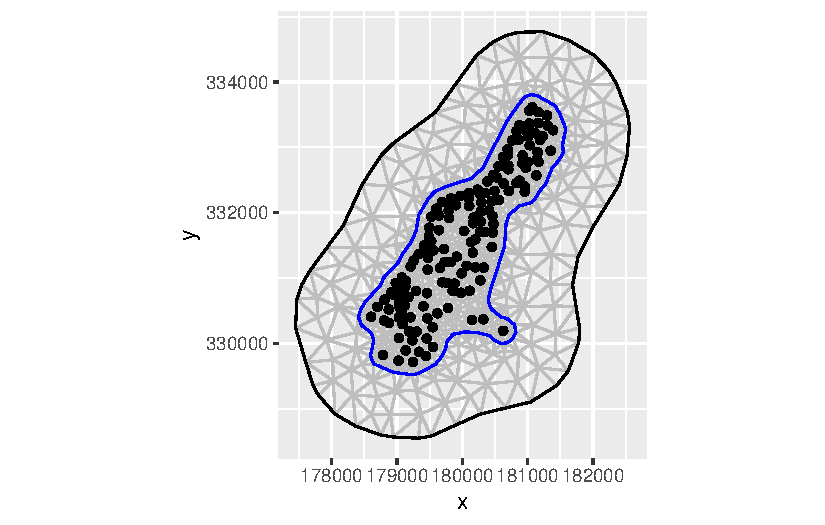
\includegraphics{pedometron_files/figure-pdf/unnamed-chunk-4-1.pdf}

}

\end{figure}

\hypertarget{defining-the-spatial-gaussian-random-field-ws}{%
\subsection{\texorpdfstring{Defining the spatial Gaussian random field
\(W(s)\)}{Defining the spatial Gaussian random field W(s)}}\label{defining-the-spatial-gaussian-random-field-ws}}

We choose the Matérn covariance function for the Gaussian random field
because it can be easily fitted in \texttt{INLA} using a SPDE. The
Matérn covariance in \texttt{INLA} depends on three parameters: - a
fractional order parameter *alpha* in the SPDE linked to the smoothness
of the solution, - a standard deviation parameter *sigma* and, - a
spatial correlation parameter known as the *range*.

We specify these parameters in our model by selecting a penalized
complexity prior using the \texttt{INLA::inla.spde2.pcmatern} function.
For more details, please refer to the introduction to spatial models
with \texttt{INLA} in chapter 7 at
\textless https://becarioprecario.bitbucket.io/inla-gitbook/ch-spatial.html\textgreater.

\begin{Shaded}
\begin{Highlighting}[]
\NormalTok{matern }\OtherTok{\textless{}{-}}
\NormalTok{  INLA}\SpecialCharTok{::}\FunctionTok{inla.spde2.pcmatern}\NormalTok{(mesh,}
                      \AttributeTok{alpha =} \DecValTok{2}\NormalTok{,}\CommentTok{\# fractional operator which is related}
                      \AttributeTok{prior.sigma =} \FunctionTok{c}\NormalTok{(}\DecValTok{1}\NormalTok{, }\FloatTok{0.5}\NormalTok{),}\CommentTok{\# P(sigma \textgreater{} 1) = 0.5}
                      \AttributeTok{prior.range =} \FunctionTok{c}\NormalTok{(}\DecValTok{10000}\NormalTok{, }\FloatTok{0.9}\NormalTok{)  }\CommentTok{\# P(range \textless{} 10000 m) = 0.9}
\NormalTok{  )}
\end{Highlighting}
\end{Shaded}

\hypertarget{specify-the-hierarchical-model}{%
\subsection{Specify the hierarchical
model}\label{specify-the-hierarchical-model}}

We then specify, in \texttt{cmp}, the model components using the
convinient \texttt{INLA\ Bru} approach. We use as example the following
latent effects: intercept, a linear relationship with the covariate
corresponding to the distance to the river, and the Gaussian random
field.

\begin{Shaded}
\begin{Highlighting}[]
\NormalTok{cmp }\OtherTok{\textless{}{-}}\NormalTok{ om }\SpecialCharTok{\textasciitilde{}} 
  \FunctionTok{field}\NormalTok{(coordinates, }\AttributeTok{model =}\NormalTok{ matern ) }\SpecialCharTok{+} 
  \FunctionTok{Intercept}\NormalTok{(}\DecValTok{1}\NormalTok{) }\SpecialCharTok{+} 
  \FunctionTok{dist}\NormalTok{(dist, }\AttributeTok{model =} \StringTok{\textquotesingle{}linear\textquotesingle{}}\NormalTok{ )     }
\end{Highlighting}
\end{Shaded}

Finally, we fit the hierarchical model to the data using the
\texttt{bru} function of the \texttt{inlabru} package. This function
requires the model components defined earlier (\texttt{cmp}), the
dataset (\texttt{meuse}), , the mesh (\texttt{mesh}) where the model
will be evaluated, and several options to control the INLA algorithm.

the spatial domain where the data were collected can be aslo provided
using the (\texttt{domainSP})

We use here the \texttt{eb} strategy as it is much quicker to compute
but a bit less accurate.

\begin{Shaded}
\begin{Highlighting}[]
\NormalTok{fit }\OtherTok{\textless{}{-}}\NormalTok{ inlabru}\SpecialCharTok{::} \FunctionTok{bru}\NormalTok{(}\AttributeTok{components =}\NormalTok{ cmp,}
           \AttributeTok{data =}\NormalTok{ meuse,}
           \AttributeTok{family =} \StringTok{"gaussian"}\NormalTok{,}
           \AttributeTok{domain =} \FunctionTok{list}\NormalTok{(}\AttributeTok{coordinates =}\NormalTok{ mesh),}
           \AttributeTok{options =} \FunctionTok{list}\NormalTok{(}
             \AttributeTok{control.inla =} \FunctionTok{list}\NormalTok{(}\AttributeTok{int.strategy =} \StringTok{"eb"}\NormalTok{),}
             \AttributeTok{verbose =} \ConstantTok{FALSE}\NormalTok{)}
\NormalTok{           )}
\end{Highlighting}
\end{Shaded}

The summary gives the posterior estimates of fixed effects (intercept
and elevation) and hyperparameters (standard deviation and range of the
Gaussian random field).

We can look at some summaries of the posterior distributions for the
parameters, for example the fixed effects (i.e.~the intercept) and the
hyper-parameters (i.e.~dispersion in the gamma likelihood, the precision
of the RW1, and the parameters of the spatial field):

\begin{Shaded}
\begin{Highlighting}[]
\FunctionTok{summary}\NormalTok{(fit)}
\end{Highlighting}
\end{Shaded}

\begin{verbatim}
inlabru version: 2.7.0
INLA version: 22.12.16
Components:
field: main = spde(coordinates)
Intercept: main = linear(1)
dist: main = linear(dist)
Likelihoods:
  Family: 'gaussian'
    Data class: 'SpatialPointsDataFrame'
    Predictor: om ~ .
Time used:
    Pre = 1.3, Running = 0.847, Post = 0.0666, Total = 2.21 
Fixed effects:
             mean    sd 0.025quant 0.5quant 0.975quant    mode kld
Intercept  10.976 1.149      8.723   10.976     13.228  10.976   0
dist      -11.587 2.607    -16.696  -11.587     -6.478 -11.587   0

Random effects:
  Name    Model
    field SPDE2 model

Model hyperparameters:
                                            mean      sd 0.025quant 0.5quant
Precision for the Gaussian observations    0.338   0.084      0.203    0.328
Range for field                         1070.631 423.165    522.243  979.530
Stdev for field                            3.191   0.755      2.040    3.078
                                        0.975quant    mode
Precision for the Gaussian observations      0.532   0.309
Range for field                           2150.174 820.388
Stdev for field                              4.991   2.837

Deviance Information Criterion (DIC) ...............: 669.11
Deviance Information Criterion (DIC, saturated) ....: 217.11
Effective number of parameters .....................: 61.64

Watanabe-Akaike information criterion (WAIC) ...: 670.85
Effective number of parameters .................: 49.87

Marginal log-Likelihood:  -380.49 
 is computed 
Posterior summaries for the linear predictor and the fitted values are computed
(Posterior marginals needs also 'control.compute=list(return.marginals.predictor=TRUE)')
\end{verbatim}

\hypertarget{spatial-predictions}{%
\section{Spatial predictions}\label{spatial-predictions}}

Now we use the fit to predict the field on a lattice, and generate a set
of results using 100 realizations from the posterior distribution:

\begin{Shaded}
\begin{Highlighting}[]
\NormalTok{pred }\OtherTok{\textless{}{-}} \FunctionTok{predict}\NormalTok{(}
\NormalTok{  fit,}
  \AttributeTok{n.samples =} \DecValTok{100}\NormalTok{,}
\NormalTok{  meuse.grid,}
  \SpecialCharTok{\textasciitilde{}}\NormalTok{ field }\SpecialCharTok{+}\NormalTok{ Intercept }\SpecialCharTok{+}\NormalTok{ dist ,}
  \AttributeTok{num.threads =} \DecValTok{2}
\NormalTok{)}
\end{Highlighting}
\end{Shaded}

It is also very simple to draw samples from the posterior distribution.
Here we draw 5 samples and select the first one.

\begin{Shaded}
\begin{Highlighting}[]
\NormalTok{samp }\OtherTok{\textless{}{-}} \FunctionTok{generate}\NormalTok{(fit, }
\NormalTok{                 meuse.grid,}
                 \SpecialCharTok{\textasciitilde{}}\NormalTok{ field }\SpecialCharTok{+}\NormalTok{ Intercept }\SpecialCharTok{+}\NormalTok{ dist ,}
                 \AttributeTok{n.samples =} \DecValTok{5}
\NormalTok{)}

\FunctionTok{str}\NormalTok{(samp)}
\end{Highlighting}
\end{Shaded}

\begin{verbatim}
 num [1:3103, 1:5] 12.5 13.5 12.4 11 14.3 ...
\end{verbatim}

\begin{Shaded}
\begin{Highlighting}[]
\NormalTok{pred}\SpecialCharTok{$}\NormalTok{sample }\OtherTok{\textless{}{-}}\NormalTok{ samp[, }\DecValTok{1}\NormalTok{]}
\end{Highlighting}
\end{Shaded}

\hypertarget{plotting-results}{%
\section{Plotting results}\label{plotting-results}}

\hypertarget{the-differents-effects}{%
\subsection{The differents effects}\label{the-differents-effects}}

We can plot the posterior densities for the latent effect Intercept and
distance to the border.

To this end we will use the \texttt{inlabru::plot()} function,

\begin{Shaded}
\begin{Highlighting}[]
\FunctionTok{plot}\NormalTok{(fit, }\StringTok{"Intercept"}\NormalTok{)}
\end{Highlighting}
\end{Shaded}

\begin{figure}[H]

{\centering 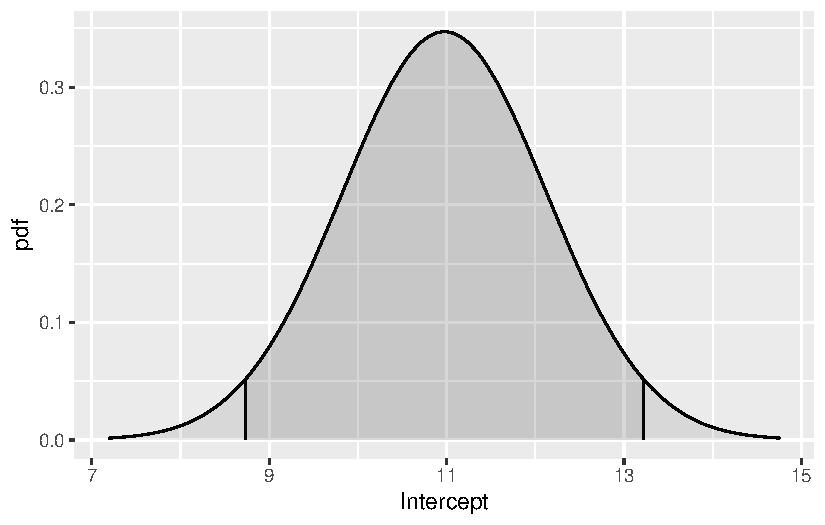
\includegraphics{pedometron_files/figure-pdf/unnamed-chunk-11-1.pdf}

}

\end{figure}

\begin{Shaded}
\begin{Highlighting}[]
\FunctionTok{plot}\NormalTok{(fit, }\StringTok{"dist"}\NormalTok{)}
\end{Highlighting}
\end{Shaded}

\begin{figure}[H]

{\centering 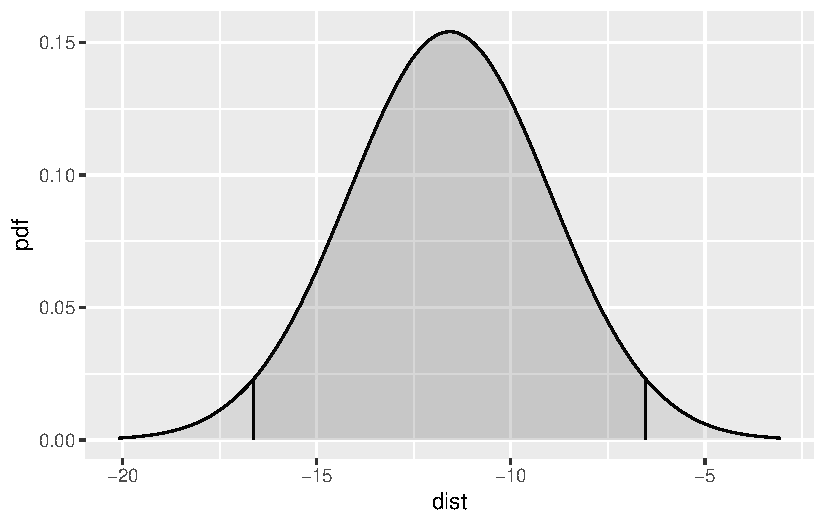
\includegraphics{pedometron_files/figure-pdf/unnamed-chunk-11-2.pdf}

}

\end{figure}

\hypertarget{the-spatial-prediction-maps-with-uncertainty}{%
\subsection{The spatial prediction maps with
uncertainty}\label{the-spatial-prediction-maps-with-uncertainty}}

You can plot the median, lower 95\% and upper 95\% density surfaces as
follows (assuming that the predicted intensity is in object
\texttt{pred}).

\begin{Shaded}
\begin{Highlighting}[]
\NormalTok{pred}\SpecialCharTok{$}\NormalTok{q0}\FloatTok{.025}\NormalTok{[pred}\SpecialCharTok{$}\NormalTok{q0}\FloatTok{.025}\SpecialCharTok{\textless{}}\DecValTok{0}\NormalTok{] }\OtherTok{=} \DecValTok{0} 

\FunctionTok{tm\_shape}\NormalTok{(pred) }\SpecialCharTok{+}
  \FunctionTok{tm\_raster}\NormalTok{(}
    \FunctionTok{c}\NormalTok{(}\StringTok{"q0.025"}\NormalTok{,}\StringTok{"median"}\NormalTok{,}\StringTok{"q0.975"}\NormalTok{)}
\NormalTok{    )}
\end{Highlighting}
\end{Shaded}

\begin{figure}[H]

{\centering 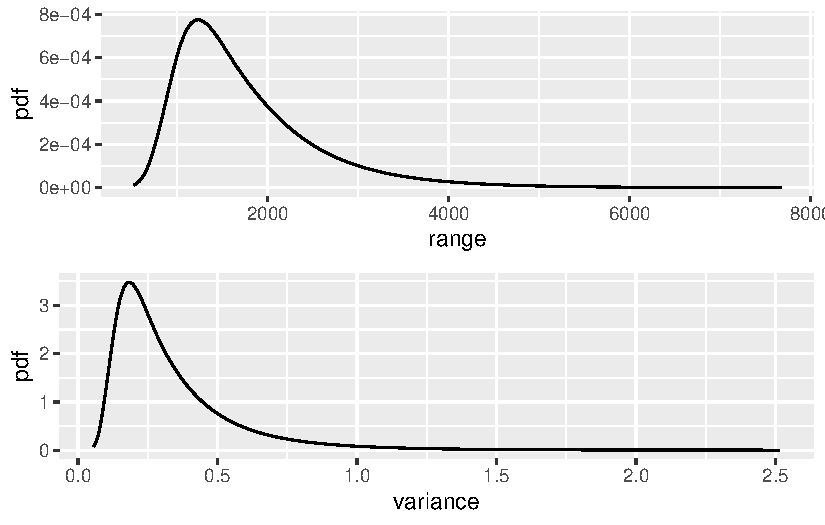
\includegraphics{pedometron_files/figure-pdf/unnamed-chunk-12-1.pdf}

}

\end{figure}

\hypertarget{one-realisation}{%
\subsection{One realisation}\label{one-realisation}}

The sample from the posterior distribution

\begin{Shaded}
\begin{Highlighting}[]
\FunctionTok{tm\_shape}\NormalTok{(pred) }\SpecialCharTok{+} \FunctionTok{tm\_raster}\NormalTok{(}\StringTok{"sample"}\NormalTok{)}
\end{Highlighting}
\end{Shaded}

\begin{figure}[H]

{\centering 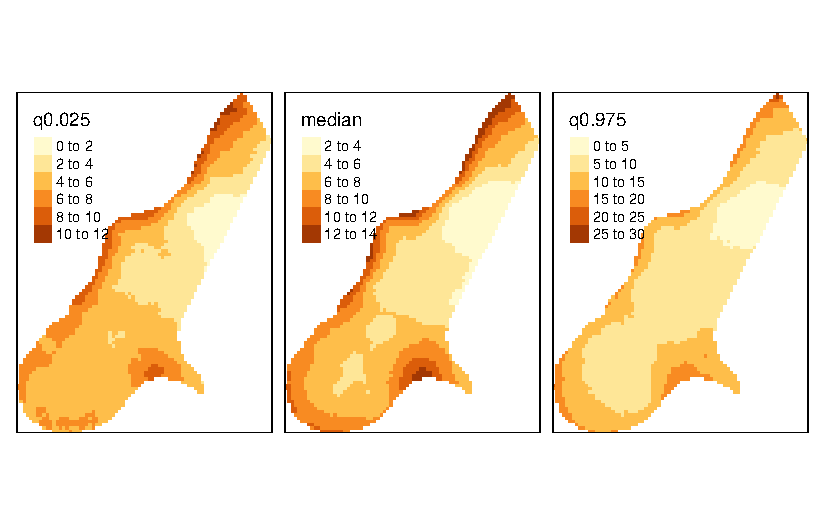
\includegraphics{pedometron_files/figure-pdf/unnamed-chunk-13-1.pdf}

}

\end{figure}

\hypertarget{the-spatial-effect}{%
\section{The spatial effect}\label{the-spatial-effect}}

We plot here the spatial Gaussian random field \(W(s)\)

\begin{Shaded}
\begin{Highlighting}[]
\NormalTok{pred }\OtherTok{\textless{}{-}} \FunctionTok{predict}\NormalTok{(}
\NormalTok{  fit,}
  \AttributeTok{n.samples =} \DecValTok{100}\NormalTok{,}
\NormalTok{  meuse.grid,}
  \SpecialCharTok{\textasciitilde{}}\NormalTok{ field  ,}
  \AttributeTok{num.threads =} \DecValTok{2}
\NormalTok{)}

\FunctionTok{tm\_shape}\NormalTok{(pred) }\SpecialCharTok{+} \FunctionTok{tm\_raster}\NormalTok{(}\StringTok{"median"}\NormalTok{)}
\end{Highlighting}
\end{Shaded}

\begin{figure}[H]

{\centering 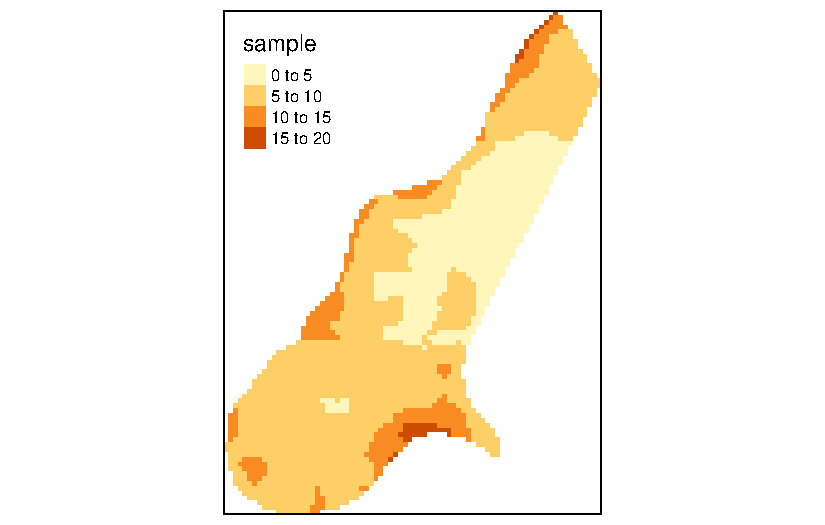
\includegraphics{pedometron_files/figure-pdf/unnamed-chunk-14-1.pdf}

}

\end{figure}

\hypertarget{rspde-fit}{%
\section{rSPDE fit}\label{rspde-fit}}

add this here ?

\begin{Shaded}
\begin{Highlighting}[]
\FunctionTok{library}\NormalTok{(rSPDE)}
\NormalTok{rspde\_model }\OtherTok{\textless{}{-}} \FunctionTok{rspde.matern}\NormalTok{(}\AttributeTok{mesh =}\NormalTok{ mesh)}
\NormalTok{cmp }\OtherTok{\textless{}{-}}\NormalTok{ om }\SpecialCharTok{\textasciitilde{}} 
  \FunctionTok{field}\NormalTok{(coordinates, }\AttributeTok{model =}\NormalTok{ rspde\_model ) }\SpecialCharTok{+} 
  \FunctionTok{Intercept}\NormalTok{(}\DecValTok{1}\NormalTok{) }\SpecialCharTok{+} 
  \FunctionTok{dist}\NormalTok{(dist, }\AttributeTok{model =} \StringTok{\textquotesingle{}linear\textquotesingle{}}\NormalTok{ )     }
\NormalTok{fit2 }\OtherTok{\textless{}{-}}\NormalTok{ inlabru}\SpecialCharTok{::} \FunctionTok{bru}\NormalTok{(}\AttributeTok{components =}\NormalTok{ cmp,}
           \AttributeTok{data =}\NormalTok{ meuse,}
           \AttributeTok{family =} \StringTok{"gaussian"}\NormalTok{,}
           \AttributeTok{domain =} \FunctionTok{list}\NormalTok{(}\AttributeTok{coordinates =}\NormalTok{ mesh),}
           \AttributeTok{options =} \FunctionTok{list}\NormalTok{(}
             \AttributeTok{control.inla =} \FunctionTok{list}\NormalTok{(}\AttributeTok{int.strategy =} \StringTok{"eb"}\NormalTok{),}
             \AttributeTok{verbose =} \ConstantTok{FALSE}\NormalTok{)}
\NormalTok{           )}
\NormalTok{result\_fit }\OtherTok{\textless{}{-}} \FunctionTok{rspde.result}\NormalTok{(fit2, }\StringTok{"field"}\NormalTok{, rspde\_model)}
\FunctionTok{summary}\NormalTok{(result\_fit)}

\NormalTok{posterior\_df\_fit }\OtherTok{\textless{}{-}} \FunctionTok{gg\_df}\NormalTok{(result\_fit)}

\FunctionTok{ggplot}\NormalTok{(posterior\_df\_fit) }\SpecialCharTok{+} \FunctionTok{geom\_line}\NormalTok{(}\FunctionTok{aes}\NormalTok{(}\AttributeTok{x =}\NormalTok{ x, }\AttributeTok{y =}\NormalTok{ y)) }\SpecialCharTok{+} 
\FunctionTok{facet\_wrap}\NormalTok{(}\SpecialCharTok{\textasciitilde{}}\NormalTok{parameter, }\AttributeTok{scales =} \StringTok{"free"}\NormalTok{) }\SpecialCharTok{+} \FunctionTok{labs}\NormalTok{(}\AttributeTok{y =} \StringTok{"Density"}\NormalTok{)}

\NormalTok{pred }\OtherTok{\textless{}{-}} \FunctionTok{predict}\NormalTok{(}
\NormalTok{  fit,}
\NormalTok{  meuse.grid,}
  \SpecialCharTok{\textasciitilde{}}\NormalTok{ field }\SpecialCharTok{+}\NormalTok{ Intercept }\SpecialCharTok{+}\NormalTok{ dist ,}
  \AttributeTok{num.threads =} \DecValTok{2}
\NormalTok{)}
\NormalTok{pred}\SpecialCharTok{$}\NormalTok{q0}\FloatTok{.025}\NormalTok{[pred}\SpecialCharTok{$}\NormalTok{q0}\FloatTok{.025}\SpecialCharTok{\textless{}}\DecValTok{0}\NormalTok{] }\OtherTok{=} \DecValTok{0} 
\FunctionTok{tm\_shape}\NormalTok{(pred) }\SpecialCharTok{+}
  \FunctionTok{tm\_raster}\NormalTok{(}
    \FunctionTok{c}\NormalTok{(}\StringTok{"q0.025"}\NormalTok{,}\StringTok{"median"}\NormalTok{,}\StringTok{"q0.975"}\NormalTok{)}
\NormalTok{    )}
\end{Highlighting}
\end{Shaded}

\hypertarget{code-availability}{%
\section{Code availability}\label{code-availability}}

The code is also available on github :
https://github.com/nsaby/pedometron042023

\hypertarget{references}{%
\section{References}\label{references}}

\hypertarget{refs}{}
\begin{CSLReferences}{1}{0}
\leavevmode\vadjust pre{\hypertarget{ref-HEUVELINK2022100639}{}}%
Heuvelink, Gerard B. M., and Richard Webster. 2022. {``Spatial
Statistics and Soil Mapping: A Blossoming Partnership Under Pressure.''}
\emph{Spatial Statistics} 50: 100639.
https://doi.org/\url{https://doi.org/10.1016/j.spasta.2022.100639}.

\leavevmode\vadjust pre{\hypertarget{ref-Huang2017}{}}%
Huang, Malone, J. 2017. {``{Evaluating a Bayesian modelling approach
(INLA-SPDE) for environmental mapping}.''} \emph{Science of The Total
Environment} 609: 621-\/-632.

\leavevmode\vadjust pre{\hypertarget{ref-Lindgren2011}{}}%
Lindgren, Finn, Håvard Rue, and Johan Lindström. 2011. {``{An explicit
link between Gaussian fields and Gaussian Markov random fields: the
stochastic partial differential equation approach}.''} \emph{Journal of
the Royal Statistical Society: Series B (Statistical Methodology)} 73
(4): 423--98.

\leavevmode\vadjust pre{\hypertarget{ref-Poggio2016}{}}%
Poggio, Laura, Alessandro Gimona, Luigi Spezia, and Mark J Brewer. 2016.
{``{Bayesian spatial modelling of soil properties and their uncertainty:
The example of soil organic matter in Scotland using R-INLA}.''}
\emph{Geoderma} 277: 69--82.

\leavevmode\vadjust pre{\hypertarget{ref-poggio_soilgrids_2021}{}}%
Poggio, L., L. M. de Sousa, N. H. Batjes, G. B. M. Heuvelink, B. Kempen,
E. Ribeiro, and D. Rossiter. 2021. {``{SoilGrids} 2.0: Producing Soil
Information for the Globe with Quantified Spatial Uncertainty.''}
\emph{SOIL} 7 (1): 217--40.
\url{https://doi.org/10.5194/soil-7-217-2021}.

\leavevmode\vadjust pre{\hypertarget{ref-Rue2009}{}}%
Rue, Håvard, Sara Martino, and Nicolas Chopin. 2009. {``{Approximate
Bayesian inference for latent Gaussian models by using integrated nested
Laplace approximations}.''} \emph{Journal of the Royal Statistical
Society: Series b (Statistical Methodology)} 71 (2): 319--92.

\leavevmode\vadjust pre{\hypertarget{ref-yuan2017point}{}}%
Yuan, Y., F. E. Bachl, F. Lindgren, D. L. Brochers, J. B. Illian, S. T.
Buckland, H. Rue, and T. Gerrodette. 2017. {``Point Process Models for
Spatio-Temporal Distance Sampling Data from a Large-Scale Survey of Blue
Whales.''} \url{https://arxiv.org/abs/1604.06013}.

\end{CSLReferences}



\end{document}
